%%%%%%%%%%%%%%%%%%%%%%%%%%%%%%%%%%%%%%%%%
% Beamer Presentation
% LaTeX Template
% Version 1.0 (10/11/12) 
%
% This template has been downloaded from:
% http://www.LaTeXTemplates.com
%
% License:
% CC BY-NC-SA 3.0 (http://creativecommons.org/licenses/by-nc-sa/3.0/)
%
%%%%%%%%%%%%%%%%%%%%%%%%%%%%%%%%%%%%%%%%%

%----------------------------------------------------------------------------------------
%	PACKAGES AND THEMES
%----------------------------------------------------------------------------------------

\documentclass{beamer}

\mode<presentation> {
%\mode<handouts> {
%\mode<article> {


% The Beamer class comes with a number of default slide themes
% which change the colors and layouts of slides. Below this is a list
% of all the themes, uncomment each in turn to see what they look like.


%\usetheme{default}
%\usetheme{AnnArbor}
%\usetheme{Antibes}
%\usetheme{Bergen}
%\usetheme{Berkeley}
%\usetheme{Berlin}
%\usetheme{Boadilla}
\usetheme{CambridgeUS}
%\usetheme{Copenhagen}
%\usetheme{Darmstadt}
%\usetheme{Dresden}
%\usetheme{Frankfurt}
%\usetheme{Goettingen}
%\usetheme{Hannover}
%\usetheme{Ilmenau}
%\usetheme{JuanLesPins}
%\usetheme{Luebeck}
%\usetheme{Madrid}
%\usetheme{Malmoe}
%\usetheme{Marburg}
%\usetheme{Montpellier}
%\usetheme{PaloAlto}
%\usetheme{Pittsburgh}
%\usetheme{Rochester}
%\usetheme{Singapore}
%\usetheme{Szeged}
%\usetheme{Warsaw}

% As well as themes, the Beamer class has a number of color themes
% for any slide theme. Uncomment each of these in turn to see how it
% changes the colors of your current slide theme.

%\usecolortheme{albatross}
\usecolortheme{beaver}
%\usecolortheme{beetle}
%\usecolortheme{crane}
%\usecolortheme{dolphin}
%\usecolortheme{dove}
%\usecolortheme{fly}
%\usecolortheme{lily}
%\usecolortheme{orchid}
%\usecolortheme{rose}
%\usecolortheme{seagull}
%\usecolortheme{seahorse}
%\usecolortheme{whale}
%\usecolortheme{wolverine}

%\setbeamertemplate{footline} % To remove the footer line in all slides uncomment this line
%\setbeamertemplate{footline}[page number] % To replace the footer line in all slides with a simple slide count uncomment this line

%\setbeamertemplate{navigation symbols}{} % To remove the navigation symbols from the bottom of all slides uncomment this line
}

\usepackage{graphicx} % Allows including images
\graphicspath{{../figures}}
\usepackage{booktabs} % Allows the use of \toprule, \midrule and \bottomrule in tables
\usepackage{amsmath, amssymb, amsthm, gensymb,mathrsfs}%,eufrak}
\usepackage{hyperref}
\usepackage{tabularx}
\usepackage{longtable}
\usepackage{makecell}
\usepackage{multicol}
\usepackage{physics}

\newcommand{\uvec}[1]{\textbf{#1}}

\newcounter{excounter}
%\renewcommand{\thefpcounter}{\thechapter.\arabic{fpcounter}}
%\renewcommand{\thefpcounter}{\thesection.\arabic{fpcounter}}
\renewcommand{\theexcounter}{\arabic{excounter}}

\newtheorem{teorema}{Teorema}[section]
\newtheorem{definicio}{Definició}[section]

\usepackage[lastexercise]{exercise}

\graphicspath{{../figures}}

%----------------------------------------------------------------------------------------
%	 TITLE PAGE
%----------------------------------------------------------------------------------------

\title[Sttatistical Learning]{Statistical Learning} % The short title appears at the bottom of every slide, the full title is only on the title page

\author{Jordi Villà i Freixa} % Your name
\institute[FCTE] % Your institution as it will appear on the bottom of every slide, may be shorthand to save space
{
Universitat de Vic - Universitat Central de Catalunya \\
Study Abroad\\ % Your institution for the title page
\medskip
\textit{jordi.villa@uvic.cat} % Your email address
}
%\date{\today} % Date, can be changed to a custom date
\date{course 2023-2024}
\logo{
\includegraphics[width=.1\textwidth]{FCTE}}
\begin{document}

\begin{frame}
\titlepage % Print the title page as the first slide
\end{frame}

\begin{frame}
\frametitle{Índex} % Table of contents slide, comment this block out to remove it
\tableofcontents % Throughout your presentation, if you choose to use \section{} and \subsection{} commands, these will automatically be printed on this slide as an overview of your presentation
\end{frame}

%----------------------------------------------------------------------------------------
%	PRESENTATION SLIDES
%----------------------------------------------------------------------------------------
\section{Introduction and scope}
\begin{frame}
  \frametitle{Preliminary note}
  The material in these slides is strongly based on \cite{kroese2020}. When other materials are used, they are cited accordingly.

  Mathematical notation follows as good as it can a \href{https://ctan.math.utah.edu/ctan/tex-archive/macros/latex/contrib/mlmath/mlmath.pdf}{good practices proposal} from the Beijing Academy of Artificial Intelligence.
  \end{frame}

%------------------------------------------------
\section{Introduction} % Sections can be created in order to organize your presentation into discrete blocks, all sections and subsections are automatically printed in the table of contents as an overview of the talk
%------------------------------------------------

%\subsection{Subsection Example} % A subsection can be created just before a set of slides with a common theme to further break down your presentation into chunks

\begin{frame}{What to expect?}
  In this session we will discuss:
  \begin{itemize}
    \item Modelling data.
    \item Models with independent and identically distributed (iid) data.
    \item The modelling dilemma.
    \item Loss function and risk.
    \item Polynomial regression.
  \end{itemize}
\end{frame}

\section{Statistical modelling}

\begin{frame}
\frametitle{How is data analyzed and used?}


\begin{description}
  \item [Statistical learning] interpret the model and quantify the uncertainity of the data.
  \item [Machine learning] (or {\em data mining}) making predictions using large scale data.
\end{description}

The goals of modelling data are:
\begin{itemize}
  \item to predict data, based on existing one;
  \item to discover unusual or interesting patterns in data. 
\end{itemize}

\end{frame}

\begin{frame}
  \frametitle{Types of machine learning}
    
    \begin{figure}
      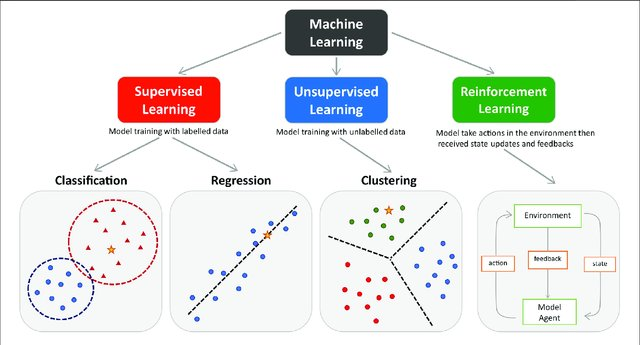
\includegraphics[width=0.9\linewidth]{MLtypes}
      \caption{Different types of machine learning techniques\cite{peng_machine_2021}}
      \label{fig:MLtypes}
    \end{figure}
  
  \end{frame}

\section{Modelling data}


\begin{frame}
  \frametitle{Supervised vs unsupervised}
    
    \begin{figure}
      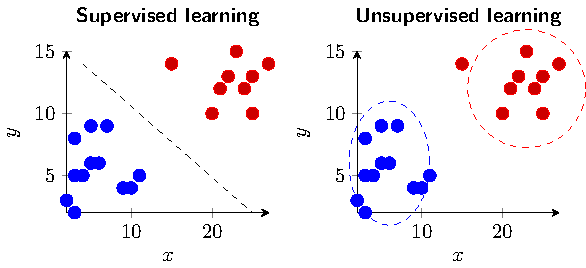
\includegraphics{supervised_unsupervised}
      \caption{Supervised vs unsupervised ML}
      \label{fig:supunsup}
    \end{figure}
  
  \end{frame}

\begin{frame}[allowframebreaks]{Example of modelling data}
  \label{sld:model}
  Imagine an unsupervised learning problem, with data represented by a vector $\bm{x}=[x_1,\ldots,x_p]^\intercal$, a very general model is to assume that $\bm{x}$ is the outcome of a random vector $\bm{X}=[X_1,\ldots,X_p]^\intercal$ with some unknown pdf $f$.\\[2ex]
 
  The model can be refined by assuming a specific form of $f$.

  \begin{figure}
    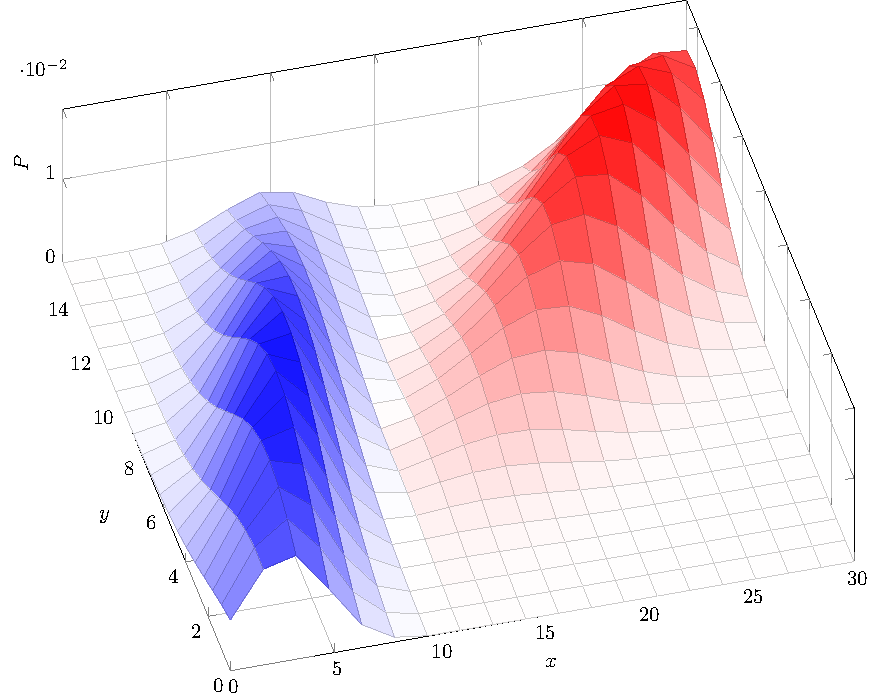
\includegraphics[width=0.5\linewidth]{2dbivariate}
    \caption{Some unknown pdf $f$ from which data in Figure \ref{fig:supunsup} was sampled.}
    \label{fig:supunsup}
  \end{figure}
\end{frame}

\begin{frame}{Example of unsupervised modelling}
  \begin{Exercise}[title={Unsupervised learning}]
    Using the data in the file, try to find 3 clusters using the K-means method.
    \begin{center}
     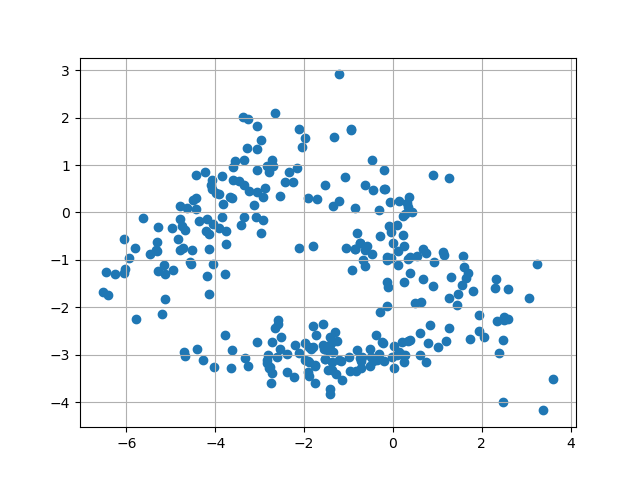
\includegraphics[width=0.6\linewidth]{data}
    \end{center}
  \end{Exercise}
\end{frame}
%------------------------------------------------

\begin{frame}
\frametitle{Tools to model data}

\begin{description}
  \item [Function approximation] Model data with approximate and simple functions or maps.
  \item [Optimization] Given a set of feasible mathematical models to the data, we may need to find the optimal one by fitting or callibrating a function to observed data.
  \item [Probability and Statistics] Probability theory and statistical inference provides ways to quantify the uncertainity inherent in making predictions based on observed data.
\end{description}
\end{frame}

%-----------------------------------

\begin{frame}{{\em iid} data}
  If we are given a sequence of data vectors $\bm{x}_1,\ldots,\bm{x}_1$ one of the simplest possible models is to assume that the corresponding random vectors $\bm{X}_1,\ldots,\bm{X}_n$ are independent and identically distributed (iid). We express this as:
  \[\bm{X}_1,\ldots,\bm{X}_n \stackrel{iid}{\sim} f \]
  meaning that the random vectors form an iid sample from a pdf $f$ or sampling distribution $Dist$.

  This is the same as saying that knowing about one variable does not provide information about another variable.
\end{frame}

\begin{frame}{Independent data models}
  In independent data models, the joint density of the random vectors $\bm{X}_1,\ldots,\bm{X}_n$ is the {\em product} of the marginal ones:
  \[
    f_{\bm{X_1},\ldots,\bm{X_n}}(\bm{x}_1,\ldots,\bm{x}_n)=f(\bm{x}_1)\cdots f(\bm{x}_n)  
  \]
  The function $g(\bm{x})$, our "model" for $f(\bm{x})$, is usually specified up to a small number of parameters, corresponding to \href{common probability distributions}:
  \begin{itemize}
    \item $\mathcal{N}(\mu,\sigma^2)$
    \item $\mathrm{Bin}(n,p)$
    \item $\mathrm{Exp}(\lambda$)
  \end{itemize}
  The parameters are typically obtained from the data.
\end{frame}

\begin{frame}{Modeling dilemma}
  \begin{figure}
    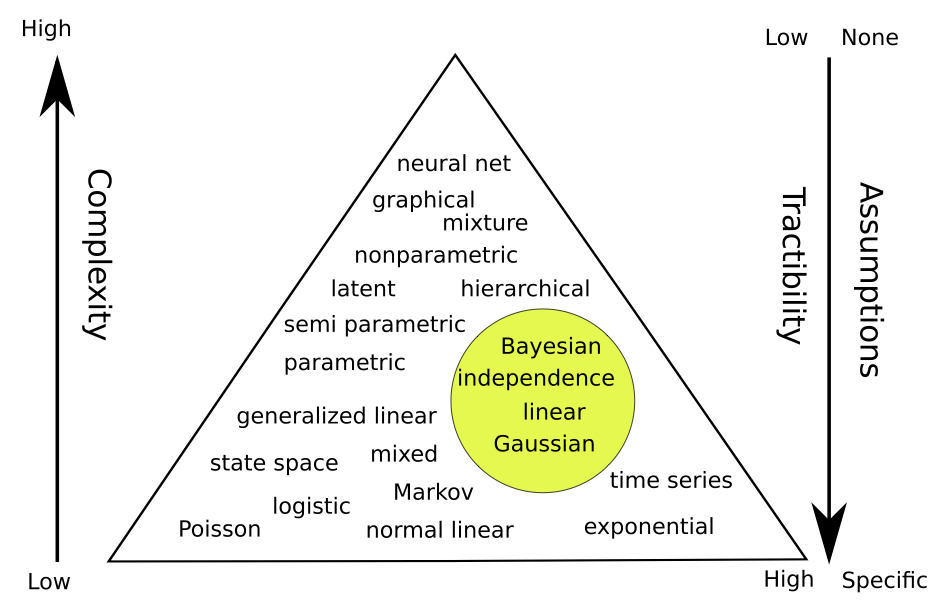
\includegraphics[width=0.7\linewidth]{dilemma}
    \caption{Complex models (very few of them) generally applicable but difficult to analyze. Simple models (a lot of options) very tractable but they do not describe well the data\cite{kroese2020}.}
    \label{fig:dilemma}
  \end{figure}
\end{frame}

\begin{frame}{Tradeoff}
  There exists a tradeoff between model tractability and applicability, as seen in Figure \ref{fig:dilemma}. Coming back to the example in page \ref{sld:model}, the {\em training set} $\tau = \{\bm{x}_1,\ldots,\bm{x}_n\}$ is viewed as the outcome of $n$ iid random variables $\bm{X}_1,\ldots,\bm{X}_n$ for some unknown pdf $f$.\\[2ex]

  {\bf Goal:} to learn or estimate $f$ from the finite training set.
\end{frame}

\begin{frame}{Tradeoff vs risk}
  Imagine the {\bf unsupervised learning} framewrok shown before. We can specify a class (a collection) of pdfs  that we will call $\mathcal{G}_p$:
  \begin{itemize}
    \item We seek within $\mathcal{G}$ the best approximation to the true model pdf $f(\bm{x}$, and we will call it $g(\bm{x}|\bm{\Theta})$. 
    \item Such best approximation will minimize some calculated risk.
  \end{itemize}
  \[
    \mathrm{Loss}(f(\bm{x}),g(\bm{x}|\bm{\Theta})))=\ln f(\bm{x}) - \ln g(\bm{x}|\bm{\Theta}))
    \]
    with expected value, this is, the {\bf risk} as
    \[
    \ell(g)= \mathbb{E}  \ln \frac{f(\bm{X})}{g(\bm{X}|\bm{\Theta})} = \int f(\bm{x}) \ln \frac{f(\bm{x})}{g(\bm{x}|\bm{\Theta})} \diff \bm{x}
    \]
\end{frame}

\begin{frame}{Train-Test-Validate}
  \begin{figure}
    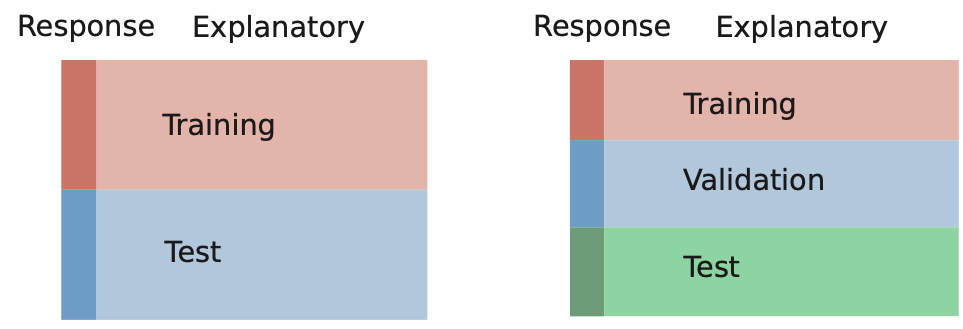
\includegraphics[width=0.7\linewidth]{traintestvalidate}
    \caption{Sometimes we use the second set of data for model validation. Then we need to use a third one for testing.}
    \label{fig:ttv}
  \end{figure}
\end{frame}

\begin{frame}{Train-Test-Validate}
  To compare the predictive performance of various learners in $\mathcal{G}$, as measured by the test loss,
  \begin{itemize}
    \item  we can use the same fixed training set $\tau$ and test set $\tau'$ for different learners, or
    \item if the overall data set is of modest size, we can perform the validation phase (model selection) on the training set only, using {\bf cross-validation}. 
  \end{itemize}

\end{frame}

\begin{frame}{Polynomial regression. Original data.}
  \begin{figure}
    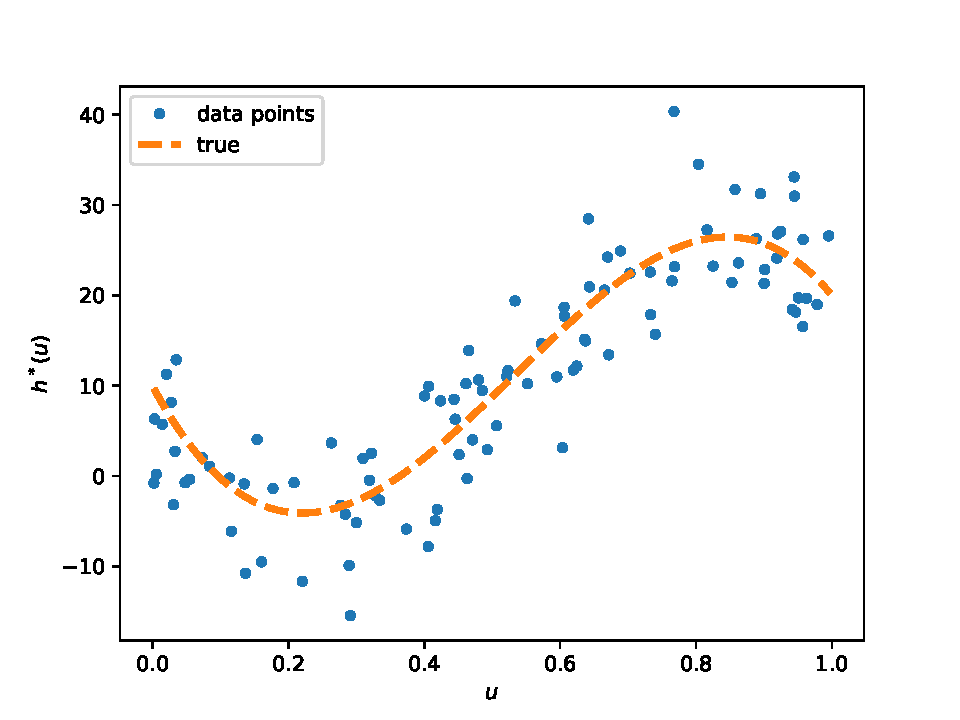
\includegraphics[width=0.7\linewidth]{polydatpy}
    \label{fig:polydatpy}
    \caption{Training data and the optimal polynomial prediction function $h^*$\cite{kroese2020}.}
  \end{figure}
\end{frame}

\begin{frame}{Polynomial regression. Fitting.}
  \begin{figure}
    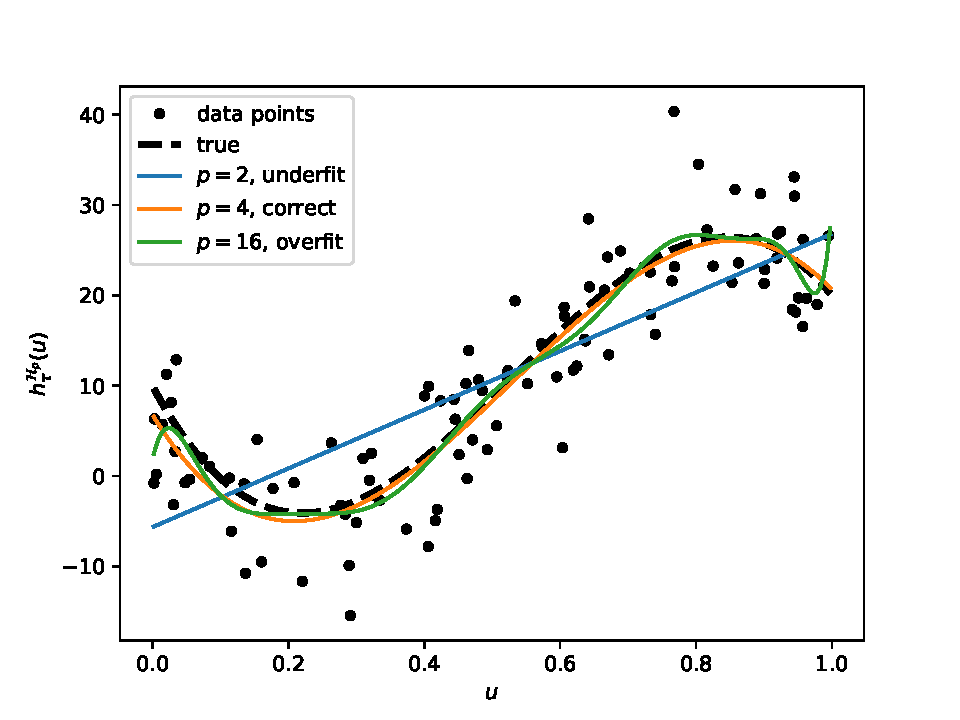
\includegraphics[width=0.7\linewidth]{polyfitpy}
    \label{fig:polydatpy}
    \caption{Fitted models for different orders of polynomial regressions\cite{kroese2020}.}
  \end{figure}
\end{frame}

\begin{frame}{Polynomial regression. Error.}
  \begin{figure}
    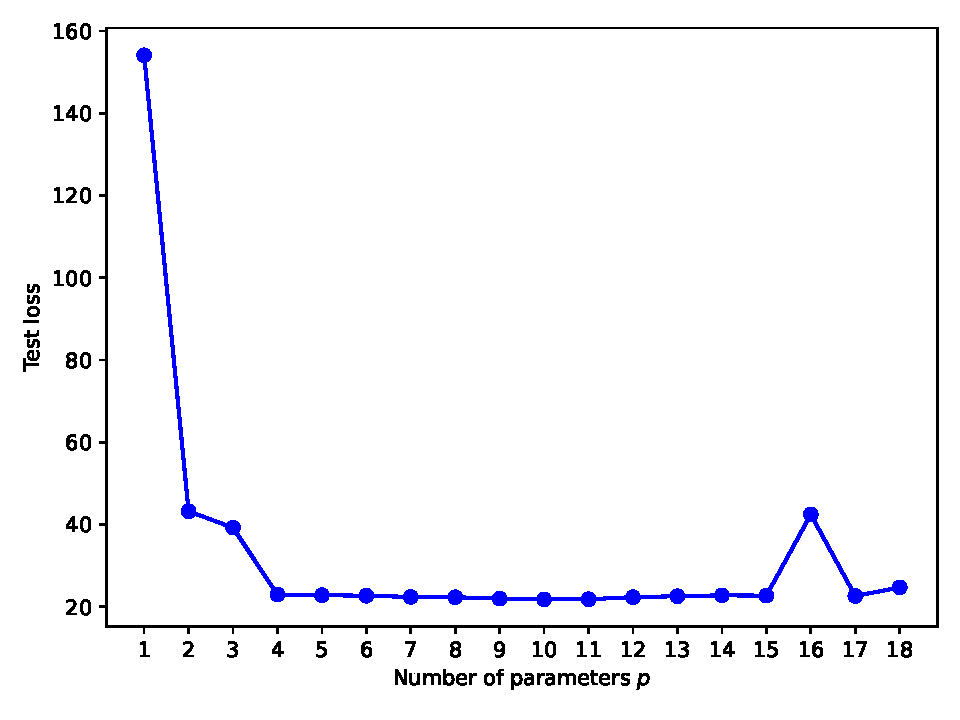
\includegraphics[width=0.7\linewidth]{MSEpy}
    \label{fig:MSEpy}
    \caption{Fitted models for different orders of polynomial regressions\cite{kroese2020}.}
  \end{figure}
\end{frame}

\begin{frame}{Polynomial regression. Cross validation.}
  \begin{figure}
    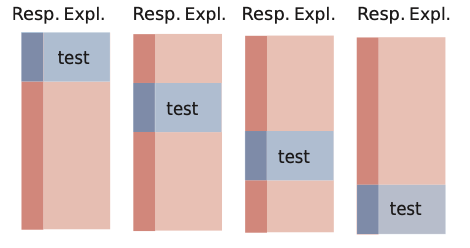
\includegraphics[width=0.4\linewidth]{crossval}
    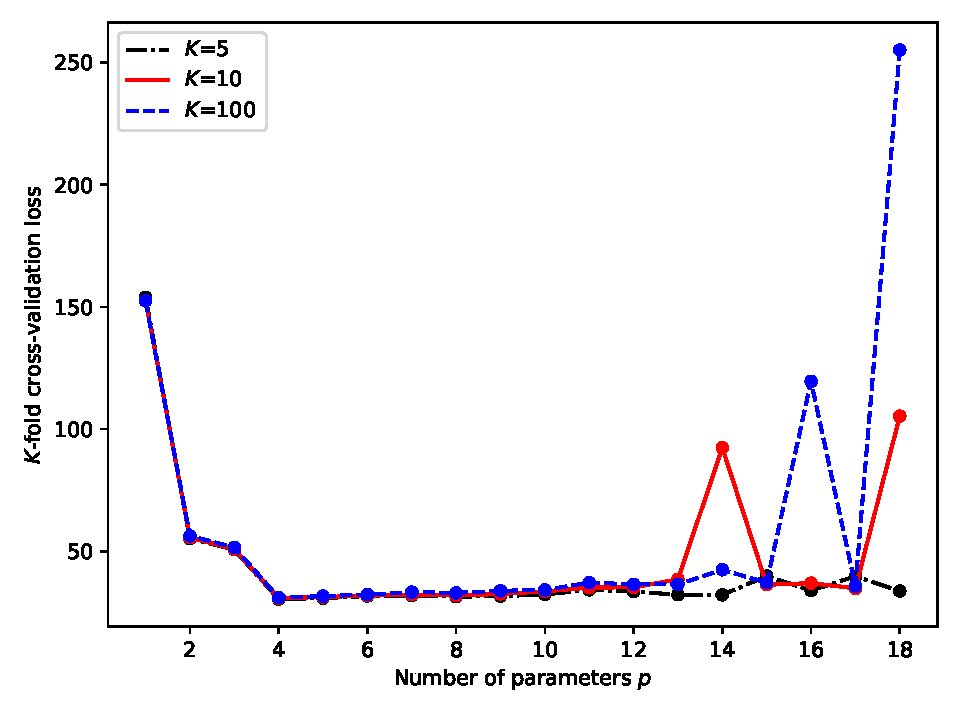
\includegraphics[width=0.4\linewidth]{crossvalpy}
    \label{fig:crossvalpy}
    \caption{a) Example of four-fold cross-validation, representing four copies of the same data set. The data in each copy is partitioned into a training set (pink) and a test set (blue).  Darker columns are the response variable; and lighter ones the explanatory variables. b) K-fold cross-validation for the polynomial regression\cite{kroese2020}.}
  \end{figure}
\end{frame}

\section{Bibliography}
\bibliographystyle{unsrt}
\bibliography{DataSciencewithPython}

\section{Detailed notation}

\begin{frame}[allowframebreaks]
  \frametitle{Annex: detailed notation}

  Given an input or {\em feature} vector $\bm{x}$, ML aims at predicting an ouput or {\em response} variable vector $\bm{y}$. In particular, we search for a mathematical {\em prediction function} $g$ such that we can {\em guess} an approximation to $\bm{y}$, $\hat{\bm{y}}$:
  \begin{align*}
      g \colon \mathcal{X}  & \rightarrow \mathcal{Y}\\
      \bm{x}                &\mapsto \hat{\bm{y}}=g(\bm{x})
  \end{align*}

  \begin{definition}
    Dataset  $S=\{\vz_i\}_{i=1}^n=\{(\vx_i,\vy_i)\}_{i=1}^n$ is sampled from a distribution $\fD$ over a domain $\fZ=\fX\times\fY$.\\
    $\fX$  is the instance domain (a set), $\fY$ is the label domain (a set), and $\fZ=\fX\times\fY$ is the example domain (a set).
  \end{definition}
  
  Usually,
  $\fX$ is a subset of $\sR^d$ and $\fY$ is a subset of $\sR^{d_{o}}$, where $d$ is the input dimension, $d_{o}$ is the output dimension.
  
  $n=\#S$ is the number of samples. Without specification, $S$ and $n$ are for the training set.

  \begin{itemize}
    \item In {\em regression} problems, $\bm{y}$ is a vector of real values.
    \item In {\em classification} problems, $\bm{y}$ values lie within a finite set of $c$ categories: $y\in\{0, 1, \ldots, c-1\}$.
  \end{itemize}

  \begin{definition}  
  A hypothesis space is denoted by $\fH$. A hypothesis function is denoted by $f_{\vtheta}(\vx)\in\fH$ or $f(\vx;\vtheta)\in\fH$ with $f_{\vtheta}:\fX\to\fY$.
  \end{definition}
  
  $\vtheta$  denotes the set of parameters of $f_{\vtheta}$.
  
  If there exists a target function, it is denoted by $f^*$or $f:\fX\to\fY$ satisfying $\vy_i=f^*(\vx_i)$ for $i=1,\ldots,n$.
  
  A loss function, denoted by $\ell:\fH\times\fZ\to\sR_+:=[0,+\infty)$, measures the difference (or error) between a predicted label and a true label, e.g., $L^2$ loss:
  \[
      \ell(f_{\vtheta},\vz)=\frac{1}{2}(f_{\vtheta}(\vx)-\vy)^2,
  \]
  where $\vz=(\vx,\vy)$. $\ell(f_{\vtheta},\vz)$ can also be written as
  \[
      \ell(f_{\vtheta}(\vx),\vy)
  \]
  for convenience.
  
  (In the case of a classification, $\ell(f_{\vtheta},\vy)=\mathbbm{1}\{y\neq \hat{\vy}\}$)

We will see other useful loss functions (\{em cross entropy\} or {\em hinge} loss functions) later in this course.

It is unlikely that a mathematical function $g \equiv \ f_{\vtheta}:\fX\to\fY$ would be able to make accurate predictions of all possible pairs $\fZ=\fX\times\fY$.

  So, we use a probabilistic approach here to mpirical risk or training loss for a set $S=\{(\vx_i,\vy_i)\}_{i=1}^{n}$ is denoted by  $\LS(\vtheta)$ or $L_{n}(\vtheta)$ or $R_{n}(\vtheta)$ or $R_{S}(\vtheta)$,
  \begin{equation}
      \LS(\vtheta) =\frac{1}{n}\sum_{i=1}^n\ell(f_{\vtheta}(\vx_i),\vy_i).
  \end{equation}
  
  The population risk or expected loss is denoted by $L_{\fD}(\vtheta)$ or $R_{\fD}(\vtheta)$
  \begin{equation}
      \LD(\vtheta) =\Exp_{\fD}\ell(f_{\vtheta}(\vx),\vy),
  \end{equation}
  where $\vz=(\vx,\vy)$ follows the distribution $\fD$.
   
  (In the case of a classification, we denote $\LD(g) \equiv \LD(\vtheta) = \Prob_{\fD} [f_{\vtheta}(\vx) \neq \vy]$ and we say that $g$ is a classifier.)

  Because we are interested in minimizing the risk in our prediction, we are looking for the best possible $g^* \colon = \mathrm{argmin}_g \Exp_{\fD}\ell(f_{\vtheta}(\vx),\vy)$

  (In classification, we look for $g^* (\vx) = \underset{y\in\{0,1,\ldots,c-1\}}{\mathrm{argmax}}  \Prob[Y=y \ X=x]$.)

  \begin{theorem}
    For the squared-error loss $\ell (y,\hat{y})=(y-\hat{y})^2$, the optimal prediction function $g^*$ is equal to the conditional expectation of $Y$ given $\vX=\vx$.
  \end{theorem}
  which leads to write the random response $Y$ as:
  \[Y=g^*(\vx)+\varepsilon(\vx)\]
  Note that such random deviation satisfies $\Exp \varepsilon(\vx)=0$
\end{frame}


%----------------------------------------------------------------------------------------


\end{document}
